\subsection{Redpanda}

Redpanda merupakan \textit{event streaming platform}. Platform ini menyediakan infrastruktur untuk \textit{streaming real-time data}. Produsen mengirimkan data berupa \textit{event} ke Redpanda, kemudian Redpanda menyimpan \textit{event} tersebut lalu mengaturnya ke dalam sebuah topik. Topik ini merupakan log \textit{event} yang dapat diputar ulang. Konsumen mengonsumsi \textit{event} pada topik Redpanda secara asinkron \parencite{redpandaIntro}.

\begin{figure}[htbp]
    \centering
    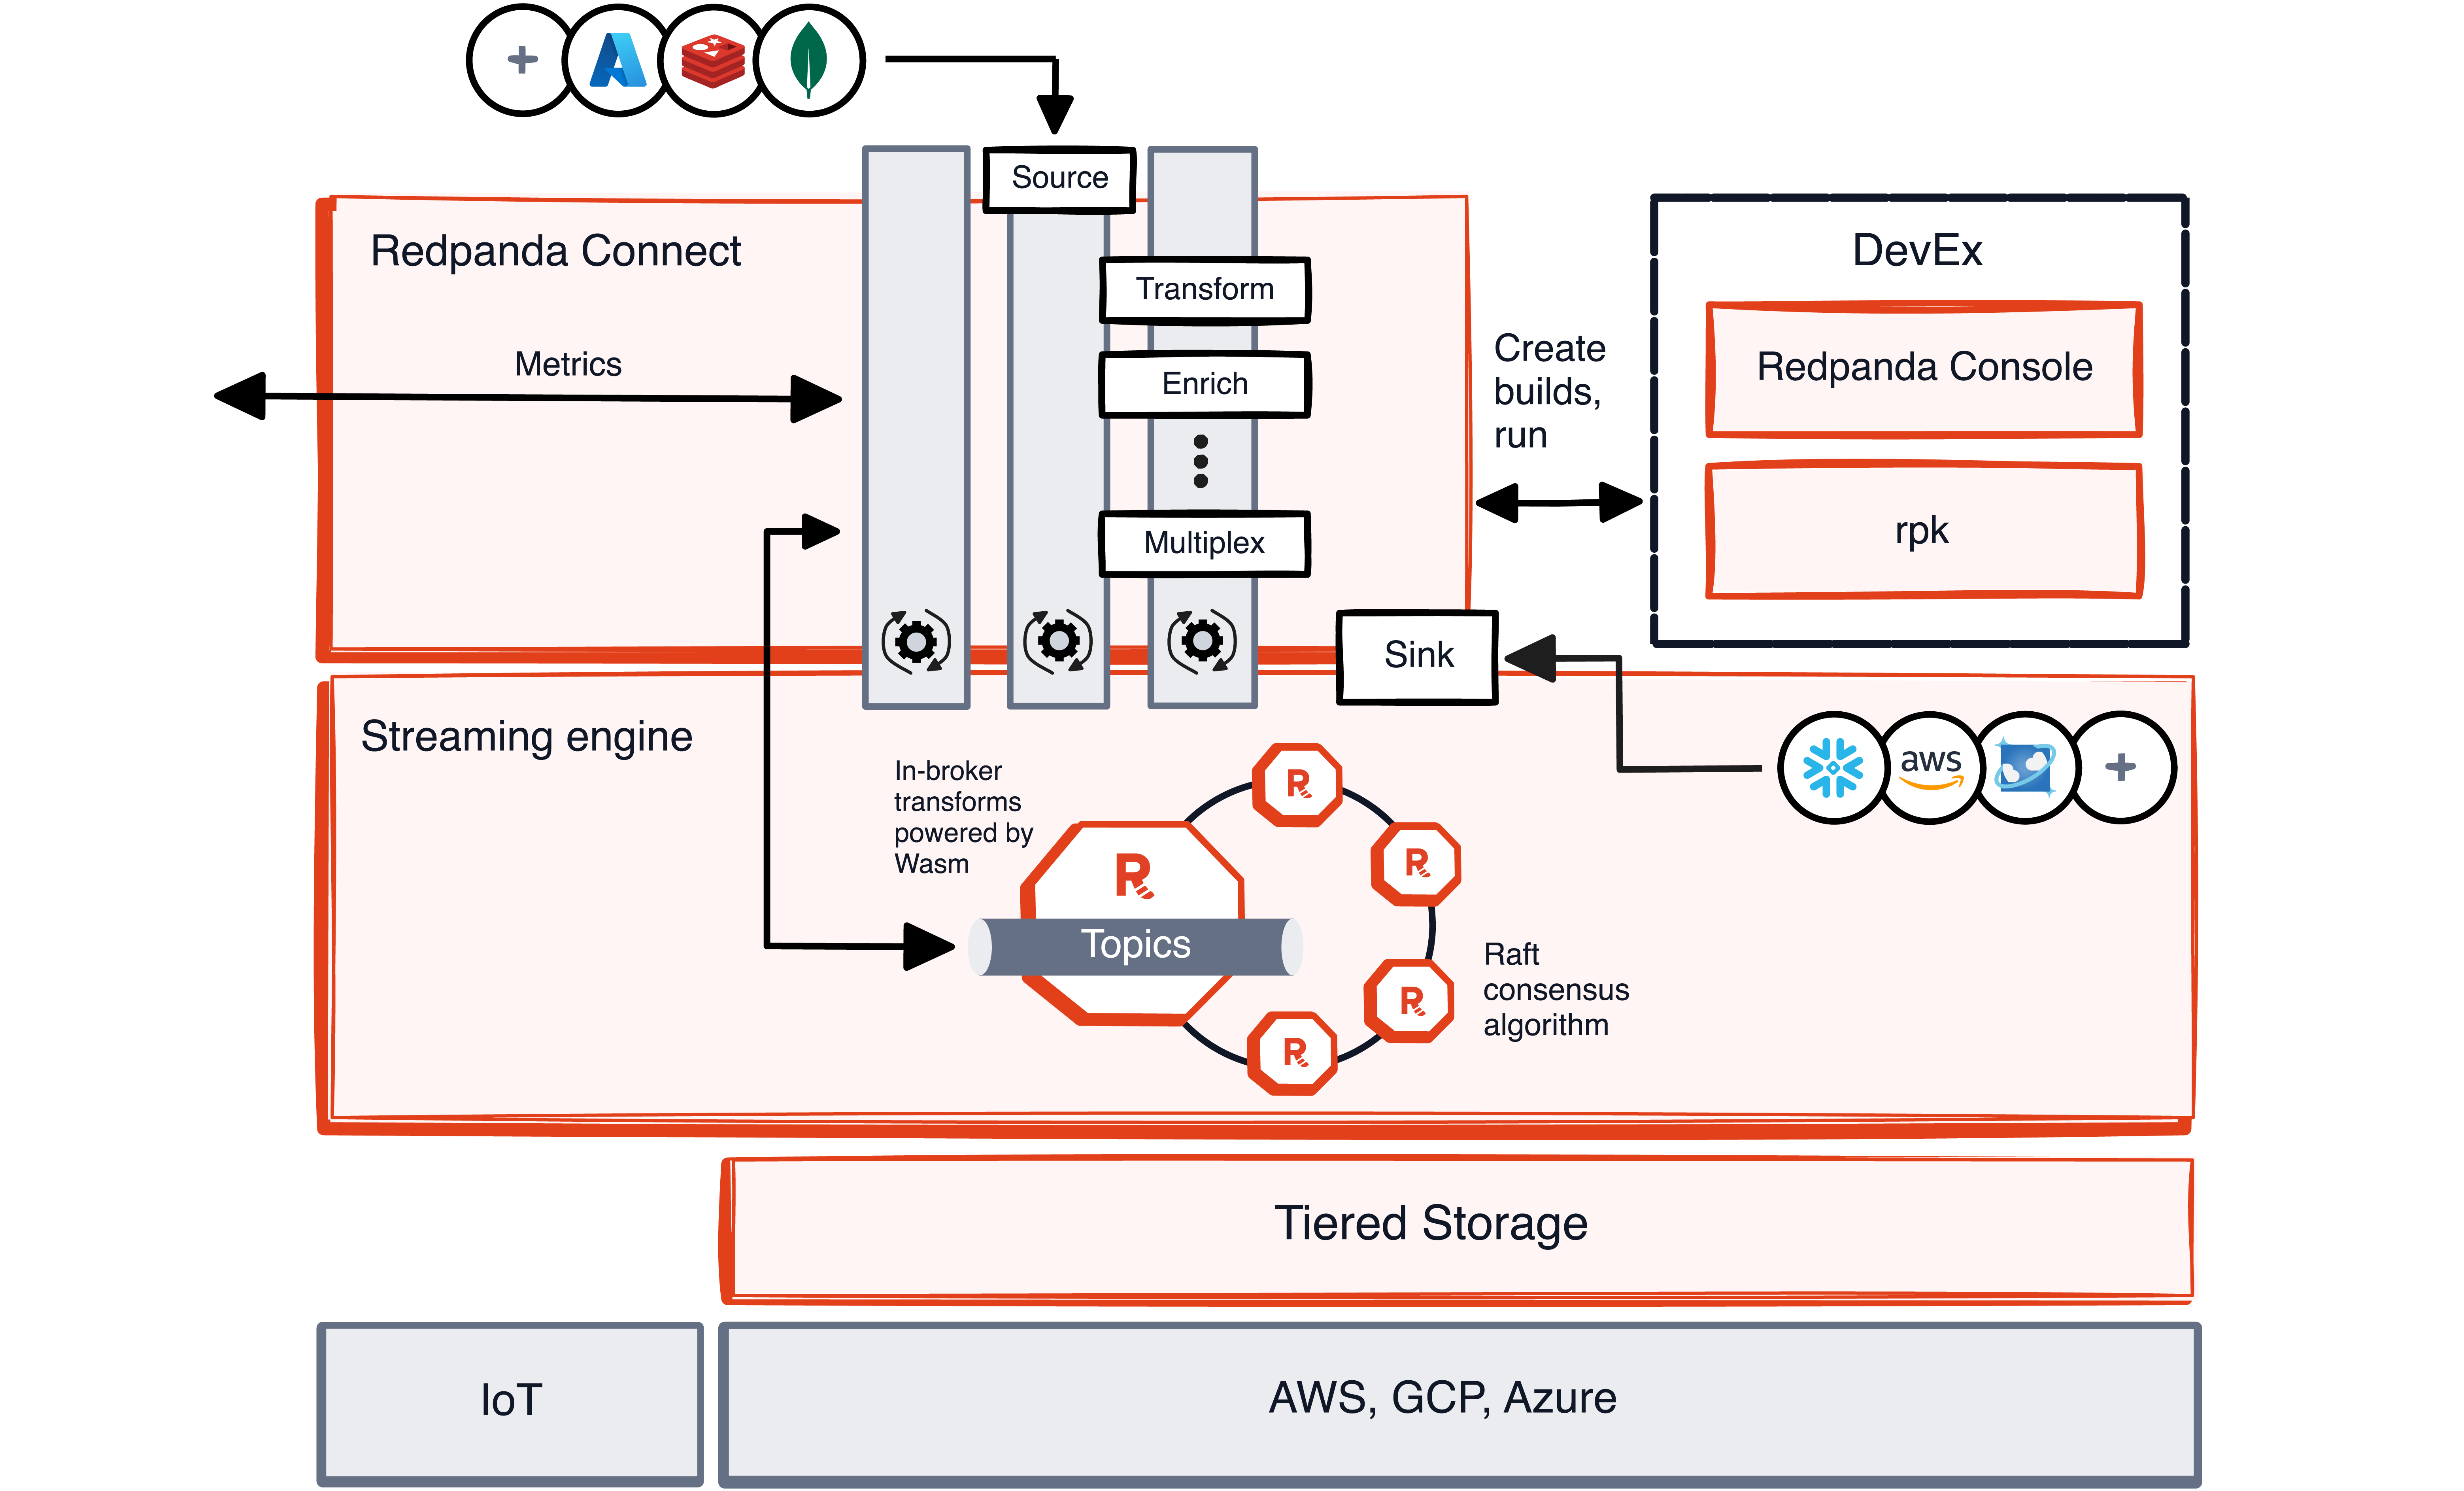
\includegraphics[width=0.8\textwidth]{resources/chapter-2/redpanda.png}
    \caption{Apa itu Redpanda? \parencite{whatIsRedpanda}}
    \label{fig:what-is-redpanda}
\end{figure}

Redpanda merupakan \textit{event streaming platform} alternatif dari Apache Kafka. Selain itu, platform ini menawarkan kompatibilitas API yang sama dengan Kafka sehingga memudahkan migrasi penggunanya. Meskipun begitu, terdapat beberapa perbedaan antara Redpanda dengan Apache Kafka.

Perbedaan pertama adalah algoritma konsensus yang digunakan. Apache Kafka menggunakan ZooKeeper (versi lama) sedangkan Redpanda menggunakan Raft. Meskipun begitu, versi terbaru Kafka sudah menggunakan algoritma konsensus Kraft yang merupakan varian dari Raft dengan perbedaan pada mekanisme replikasi log \parencite{raftKraft}.

Selain itu, Redpanda berfokus pada pengoptimalan kinerja yang lebih baik dibandingkan dengan Apache Kafka. Redpanda ditulis dalam bahasa C++, sedangkan Apache Kafka ditulis dalam bahasa Java dan berjalan pada JVM. Dalam hal ini, Redpanda menggunakan bahasa sistem sehingga minim \textit{overhead}.

Berikut adalah contoh pengoptimalan yang dilakukan pada Redpanda: \textit{Direct Memory Access (DMA)} untuk I/O, distribusi pemrosesan \textit{interrupt request} (IRQ) pada beberapa core CPU, penggunaan model \textit{thread per core}, dan pengoptimalan lainnya. Penggunaan model \textit{thread per core} memungkinkan Redpanda untuk menjalankan \textit{thread} aplikasi pada inti CPU yang sama sehingga \textit{context switching} dan \textit{blocking} dapat dihindari \parencite{redpandaArchitecture}.